\section{Metodologia}

\begin{frame}
  \frametitle{Amostragem}
  Pontos de amostragem em Nima.
  \begin{figure}[H]
    \centering
    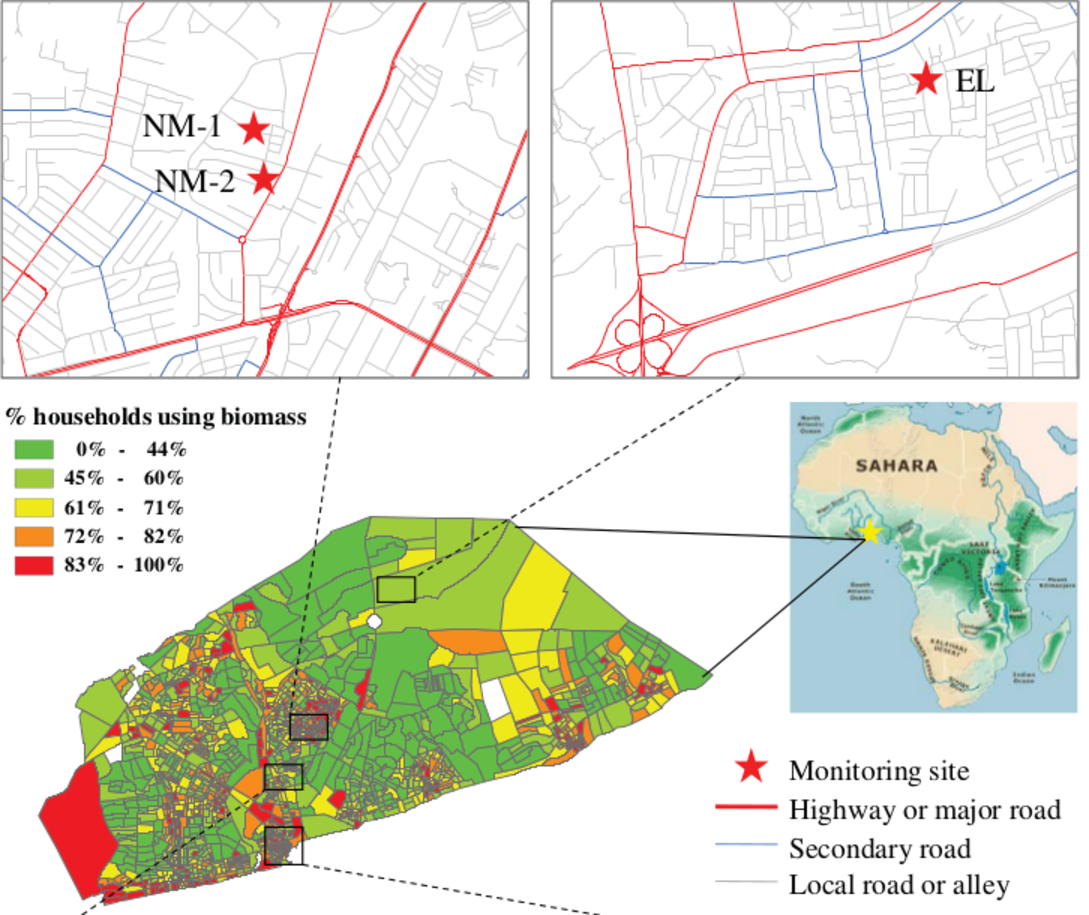
\includegraphics[scale=0.35]{../../inputs/images/zheng/nima_mapa.pdf}
  \end{figure}
\end{frame}

\begin{frame}
  \frametitle{Amostragem}
  \begin{figure}[H]
  \centering	
  \includegraphics[width=0.7\textwidth]{../../outputs/accra_sources.pdf}
  \caption{Levantamento de algumas fontes poluidora de Acra.
           \label{fg:acrasources}}
 \end{figure}
\end{frame}

\begin{frame}
  \frametitle{Análises}
  \begin{itemize}
    \item Gravimétrica (determinação da massa);  
    \item Refletância (determinação do Black Carbon);
    \item Fluorescência de Raios X (determinação da composição química inorgânica);
  \end{itemize}
\end{frame}

\begin{frame}
  \frametitle{}
  \begin{table}[H]
  	\centering
  	\begin{tabular}{llrlr}
  \hline
  \multicolumn{1}{c}{Tipo da} & \multicolumn{2}{c}{Gana (todo país)} & \multicolumn{2}{c}{Acra}                                                           \\
  \multicolumn{1}{c}{fonte de energia} & 2000 & 2010 &  2000 & 2010  \\ 
 \hline & \multicolumn{4}{c}{\% de uso} \\ 
  \hline
  não cozinha           & 3,5 & 5,60 & 4,8 & 6,90 \\ 
\textcolor{red}{biomassa}              & \textcolor{red}{55,8} & \textcolor{red}{40,20} & \textcolor{red}{8,8} & \textcolor{red}{3,50} \\ 
\textcolor{blue}{gás}& \textcolor{blue}{6,2} & \textcolor{blue}{18,20} & \textcolor{blue}{21,8} & \textcolor{blue}{41,40} \\ 
  eletricidade          & 1,1 & 0,50 & 2,2 & 0,90 \\ 
  querosene             & 2 & 0,50 & 4,3 & 1,10 \\ 
 \textcolor{red}{carvão} & \textcolor{red}{30} & \textcolor{red}{33,70} & \textcolor{red}{57,3} & \textcolor{red}{45,40} \\ 
  resíduo de plantação  & * & 0,80 & * & 0,10 \\ 
  pó de serra           & * & 0,10 & * & 0,30 \\ 
  esterco               & * & 0,00 & * & 0,10 \\ 
  outros                & 1,1 & 0,10 & 0,8 & 0,30 \\ 
  \hline
\end{tabular}


  	\caption{Percentual relativo dos tipos de fontes de energia usadas para preparação 
  		    de alimentos em Gana. 
  		\label{table:cookfuel}}
  \end{table}
\end{frame}

\begin{frame}
  \frametitle{}
  \begin{figure}[H]
    \centering
    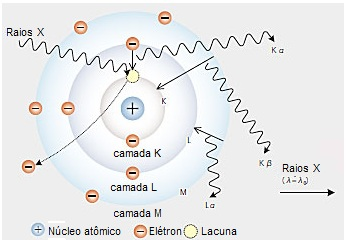
\includegraphics[width=0.5\textwidth]{../../inputs/images/shimadzu_atomo.jpg}
    \caption{Ilustração clássica do fenômeno de fluorescência de raios X no átomo. 
             Figura que acompanha o manual da Shimadzu da série de equipamentos
             EDX 700. \label{fig:shimadzu_atomo}}
  \end{figure}
\end{frame}

\begin{frame}
  \frametitle{}
  \begin{figure}[H]
    \centering 
    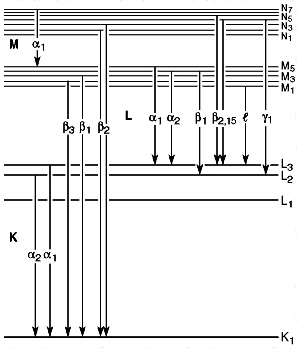
\includegraphics[width=0.5\textwidth]{../../inputs/images/Siegbahn.jpg}
    \caption{Transições de elétrons entre os subníveis das camadas K, L e M. 
             Figura extraída de. \label{fig:siegbahn}}
  \end{figure}
\end{frame}

\begin{frame}
  \frametitle{}

\end{frame}

\begin{frame}
  \frametitle{}
\end{frame}

\begin{frame}
  \frametitle{Fluorescência de Raios X - \textit{ED-XRF}}
  Modelamento matemático usado na \textit{ED-XRF}:
  \begin{equation}
    \label{eq:contagem}
    N(Z) = R(Z) \cdot I \cdot \Delta t  \cdot \frac{m(Z)}{A}
  \end{equation}
  Onde,  
  \begin{itemize}
    \item $N_{ij}$ = Contagem de fótons na amostra i para o elemento químico j;
    \item $I_{i}$ = Corrente (ampère) na amostra i;
    \item $\Delta t_i$ = Tempo vivo (segundos) que a amostra i foi irradiada;
    \item \textcolor{red}{$m_{ij}$} = Massa (grama) na amostra i para o elemento químico j;
    \item $A_i$ = Área ($cm^2$)irradiada da amostra i.
  \end{itemize}
\end{frame}

\begin{frame}
  \frametitle{Calibração: Ajuste do Fator de Resposta}
  Constante de proporcionalidade: Fator de Resposta:
\begin{equation}
  \label{eq:fator_de_resposta}
  R(Z) = \frac{N(Z)}{d(Z) \cdot I \cdot \Delta t}
\end{equation}

\begin{equation}
  \label{eq:erro_fator_de_resposta}
  \sigma_{R(Z)}^2 = {R(Z)}^2 \cdot \left( \left(\frac{\sigma_{N(Z)}}{N(Z)}\right)^2 + 
                                      \left(\frac{\sigma_{d(Z)}}{d(Z)}\right)^2 
                                   \right)
\end{equation}
%  \begin{figure}[H]
%  \centering
%    \begin{minipage}[b]{0.40\linewidth}
%      \includegraphics[scale=0.25]{../../outputs/K2014abril}
%    \end{minipage}
%    \quad
%    \begin{minipage}[b]{0.40\linewidth}
%      \includegraphics[scale=0.25]{../../outputs/L2014abril.png}
%    \end{minipage}
%  \end{figure}
\end{frame}

\begin{frame}
  \frametitle{Erro no Ajuste - Abordagem matricial mínimos quadrados}
   \begin{equation}
     [R] = A[Z]
   \end{equation}
   
   Sendo $\alpha$ o A ajustado, a covariância dos coeficientes $V_{\alpha}$:
   \begin{equation}
     V_{\alpha} = (Z^t V_R^{-1} Z)^{-1}
   \end{equation}

   O ajuste de A fica:
   \begin{equation}
     \alpha = V_{\alpha} Z^t V_R^{-1} R
   \end{equation}

    Calculando-se os novos valores de R a partir de $V_{\alpha}$:
   \begin{equation}
     [R_{adjusted}] = \alpha[Z]
   \end{equation} 

    A incerteza do ajuste é a raiz quadrada da diagonal da matriz de covariância de $R_{adjusted}$:
   \begin{equation}
     COV_{R_{adjusted}} = Z V_{\alpha} Z^t
   \end{equation} 
\end{frame}

\begin{frame}
  \frametitle{Comparação das análises com a da \textbf{EPA}}
  \begin{figure}[H]
   \centering
    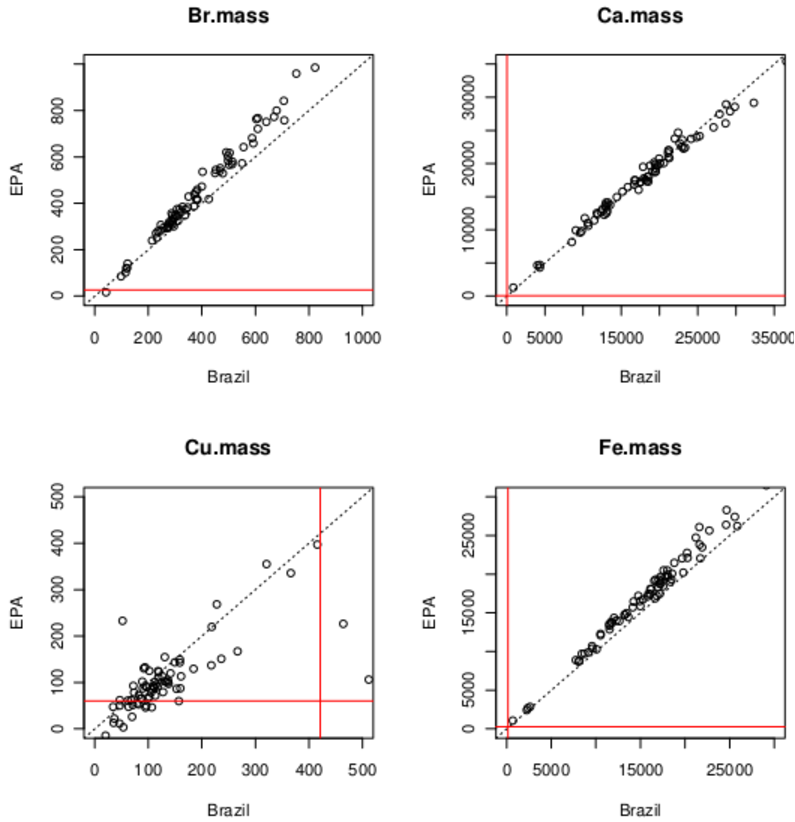
\includegraphics[scale=0.42]{../../inputs/images/zheng/epa_short_example.PDF}
  \end{figure}
  \begin{tiny}
    2900 amostras - \textbf{USP}. 
    95 de controle pela \textbf{EPA} (US Environmental Protection Agency).
  \end{tiny}
\end{frame}
\section{Metodologia}

\begin{frame}
  \frametitle{Modelo receptor}
  \textbf{Modelo Receptor} é uma abordagem matemática para quantificar o efeito das fontes 
  nas amostras. Determinar as fontes a partir do receptor. \\
  \textbf{Análise Multivariada} reduz as dimensões (variáveis) de um conjunto de dados 
  em um conjunto de dados analítico complexo que poderão ser interpretados como 
  tipo de fontes.
\end{frame}

\begin{frame}
  \frametitle{Conservação de massa}
  Fundamentação do modelo receptor: Conservação de massa. \\
  Todos modelos resolvem a mesma equação: 
  \begin{equation}
    x_{ij} = \sum_{p=1}^{P} g_{ip}f_{pj} + \epsilon_{ij}
  \end{equation} 
 
  \begin{itemize}
    \item $x_{ij}$ = concentração na amostra i da espécie j;
    \item $f_{pj}$ = fração da espécie j emitida na fonte p 
                    (perfil da fonte, assinatura da fonte ou \textit{Factor Loadings}); 
    \item $g_{ip}$ = contribuição da fonte p para amostra i (\textit{Factor Score});
    \item $\epsilon$ = Resíduo, depende do modelo empregado.
  \end{itemize}
\end{frame}

\begin{frame}
  \frametitle{Análise de Fatores}
  \begin{equation}
    z_{j} = l_{j1}F_1 + l_{j2}F_2 + l_{j3}F_3 + ... + \epsilon_{ij}
  \end{equation}
  \begin{enumerate}
    \item $z_{j}$ = concentração da espécie j normalizada;
    \item Cálculo da matriz de correlação/covariância
    \item Extração de autovalores e autovetores (ortogonais). 
    \item Transformada Linear nos novos eixos
    \item $l_{jk}$ = contribuição da Fonte $F_k$
  \end{enumerate}

\end{frame}


\begin{frame}
  \frametitle{Positive Matrix Factorizarion}

  Função objeto - Q -  é uma função que precisa ser minimizada. 
 
  \begin{equation}
    Q = \sum_{i=1}^n \sum_{j=1}^m  \left[ \frac{ x_{ij} - \sum_{p=1}^{P} g_{ip}f_{pj}} {u_{ij}} \right] ^2
  \end{equation}

  Diferente da Análise de Fatores, no PMF, a incerteza ($u_{ij}$) entra na conta.
\end{frame}

\begin{frame}
  \frametitle{}
\end{frame}
